\documentclass[tikz]{standalone}
\begin{document}
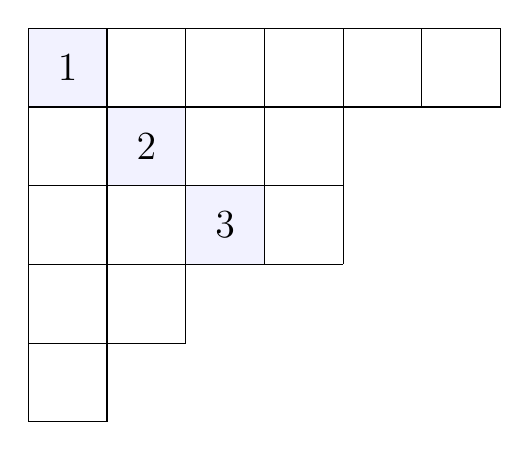
\begin{tikzpicture}
\begin{scope}[local bounding box=scope1]
  \filldraw[blue!5] (0,0) rectangle (1,-1);\filldraw[blue!5] (1,-1) rectangle (2,-2);\filldraw[blue!5] (2,-2) rectangle (3,-3);
  \draw (0,0) -- (6,0);\draw (0,-1) -- (6,-1);\draw (0,-2) -- (4,-2);\draw (0,-3) -- (4,-3);\draw (0,-4) -- (2,-4);\draw (0,-5) -- (1,-5);\draw (1,0) -- (1,-5);\draw (2,0) -- (2,-4);\draw (3,0) -- (3,-3);\draw (4,0) -- (4,-3);\draw (5,0) -- (5,-1);\draw (6,0) -- (6,-1);\draw (0,0) -- (0,-5);
\end{scope}
\begin{scope}[font=\Large, shift={(0.5,-0.5)}]
  \draw (0,0) node{1};\draw (1,-1) node{2};\draw (2,-2) node{3};
\end{scope}
\end{tikzpicture}
\end{document}
